\documentclass[../main.tex]{subfiles}

\begin{document}
Svi korisnici vide deo aplikacije za takmičenja. Neregistrovani korisnik i trener vide samo spisak predstojećih takmičenja. Ostali imaju adekvatne prorpatne dugmiće.

\begin{figure}[!ht]
\begin{center}
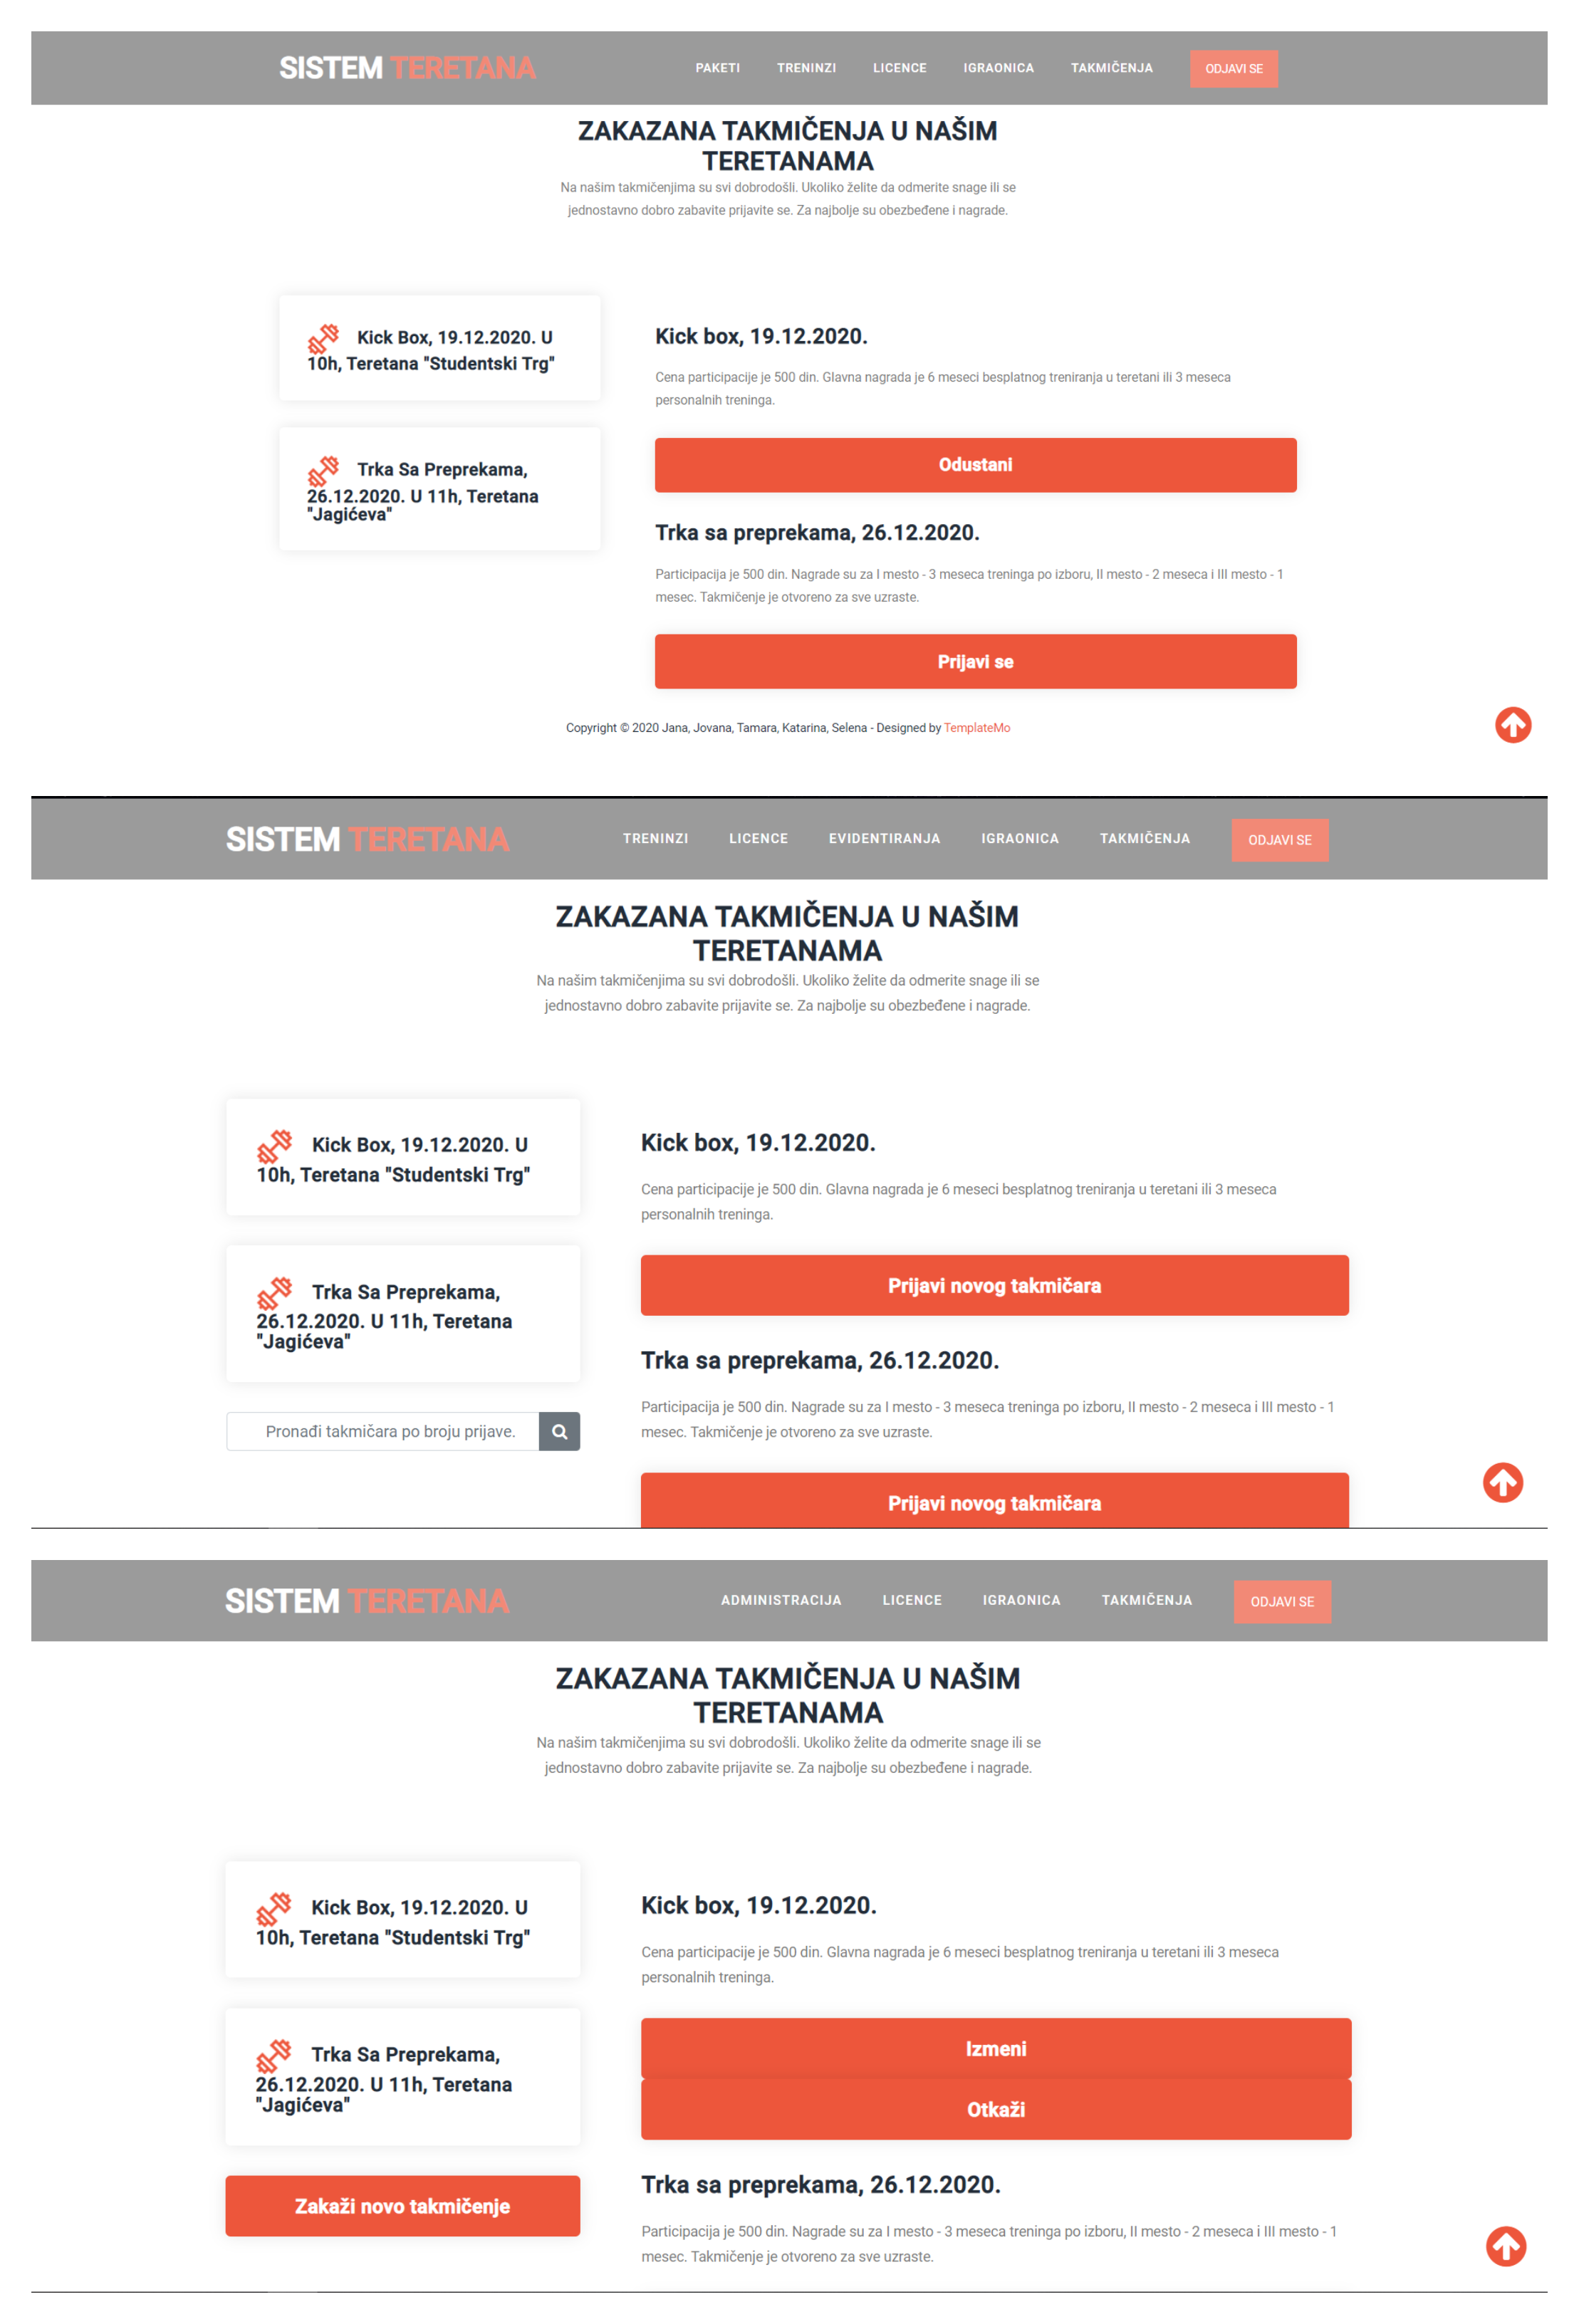
\includegraphics[scale=0.30]{sections/korisnicki_interfejs/screenshots/takmicenjaRazlUglovi.png}
\end{center}
\caption{Prikaz takmičenja iz različitih uglova odozgo nadole:  klijenta i adminitratora }
\label{fig:takmicenja_uglovi}
\end{figure}

Administrator vidi kao na slici (\ref{fig:takmicenja_uglovi} poslednja). Pritiskom na dugme Zakaži novo takmičenje otvara se formular prikazan na slici \ref{fig:t_kreiranje}. Zatim prisitkom na dugme Zakaži takmičenje otvara se prozor na slici (\ref{fig:t_kreiranje_ob} gore). Nakon kreiranog obaveštenja prikazuje obaveštenje o kreiranom tamičenju i vraća se prikaz na početnu stranu. 

\begin{figure}[!ht]
\begin{center}
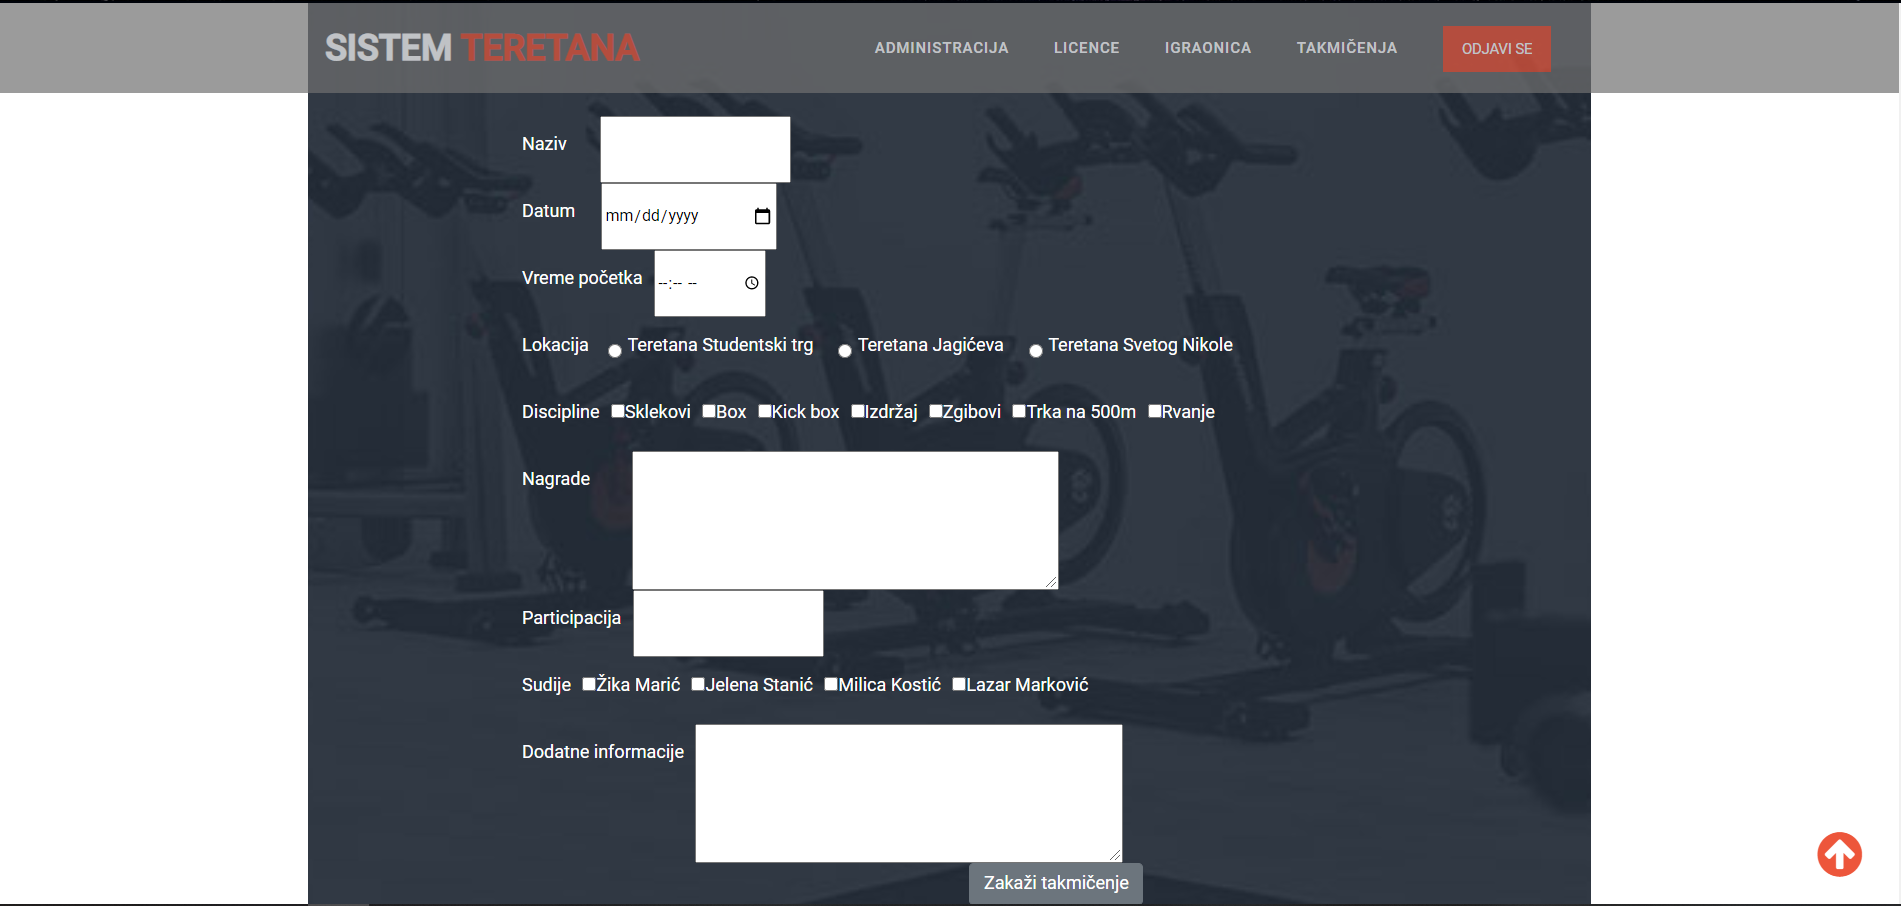
\includegraphics[scale=0.30]{sections/korisnicki_interfejs/screenshots/takmicenja_kreiranje.PNG}
\end{center}
\caption{Formular za kreiranje takmičenja}
\label{fig:t_kreiranje}
\end{figure}


\begin{figure}[!ht]
\begin{center}
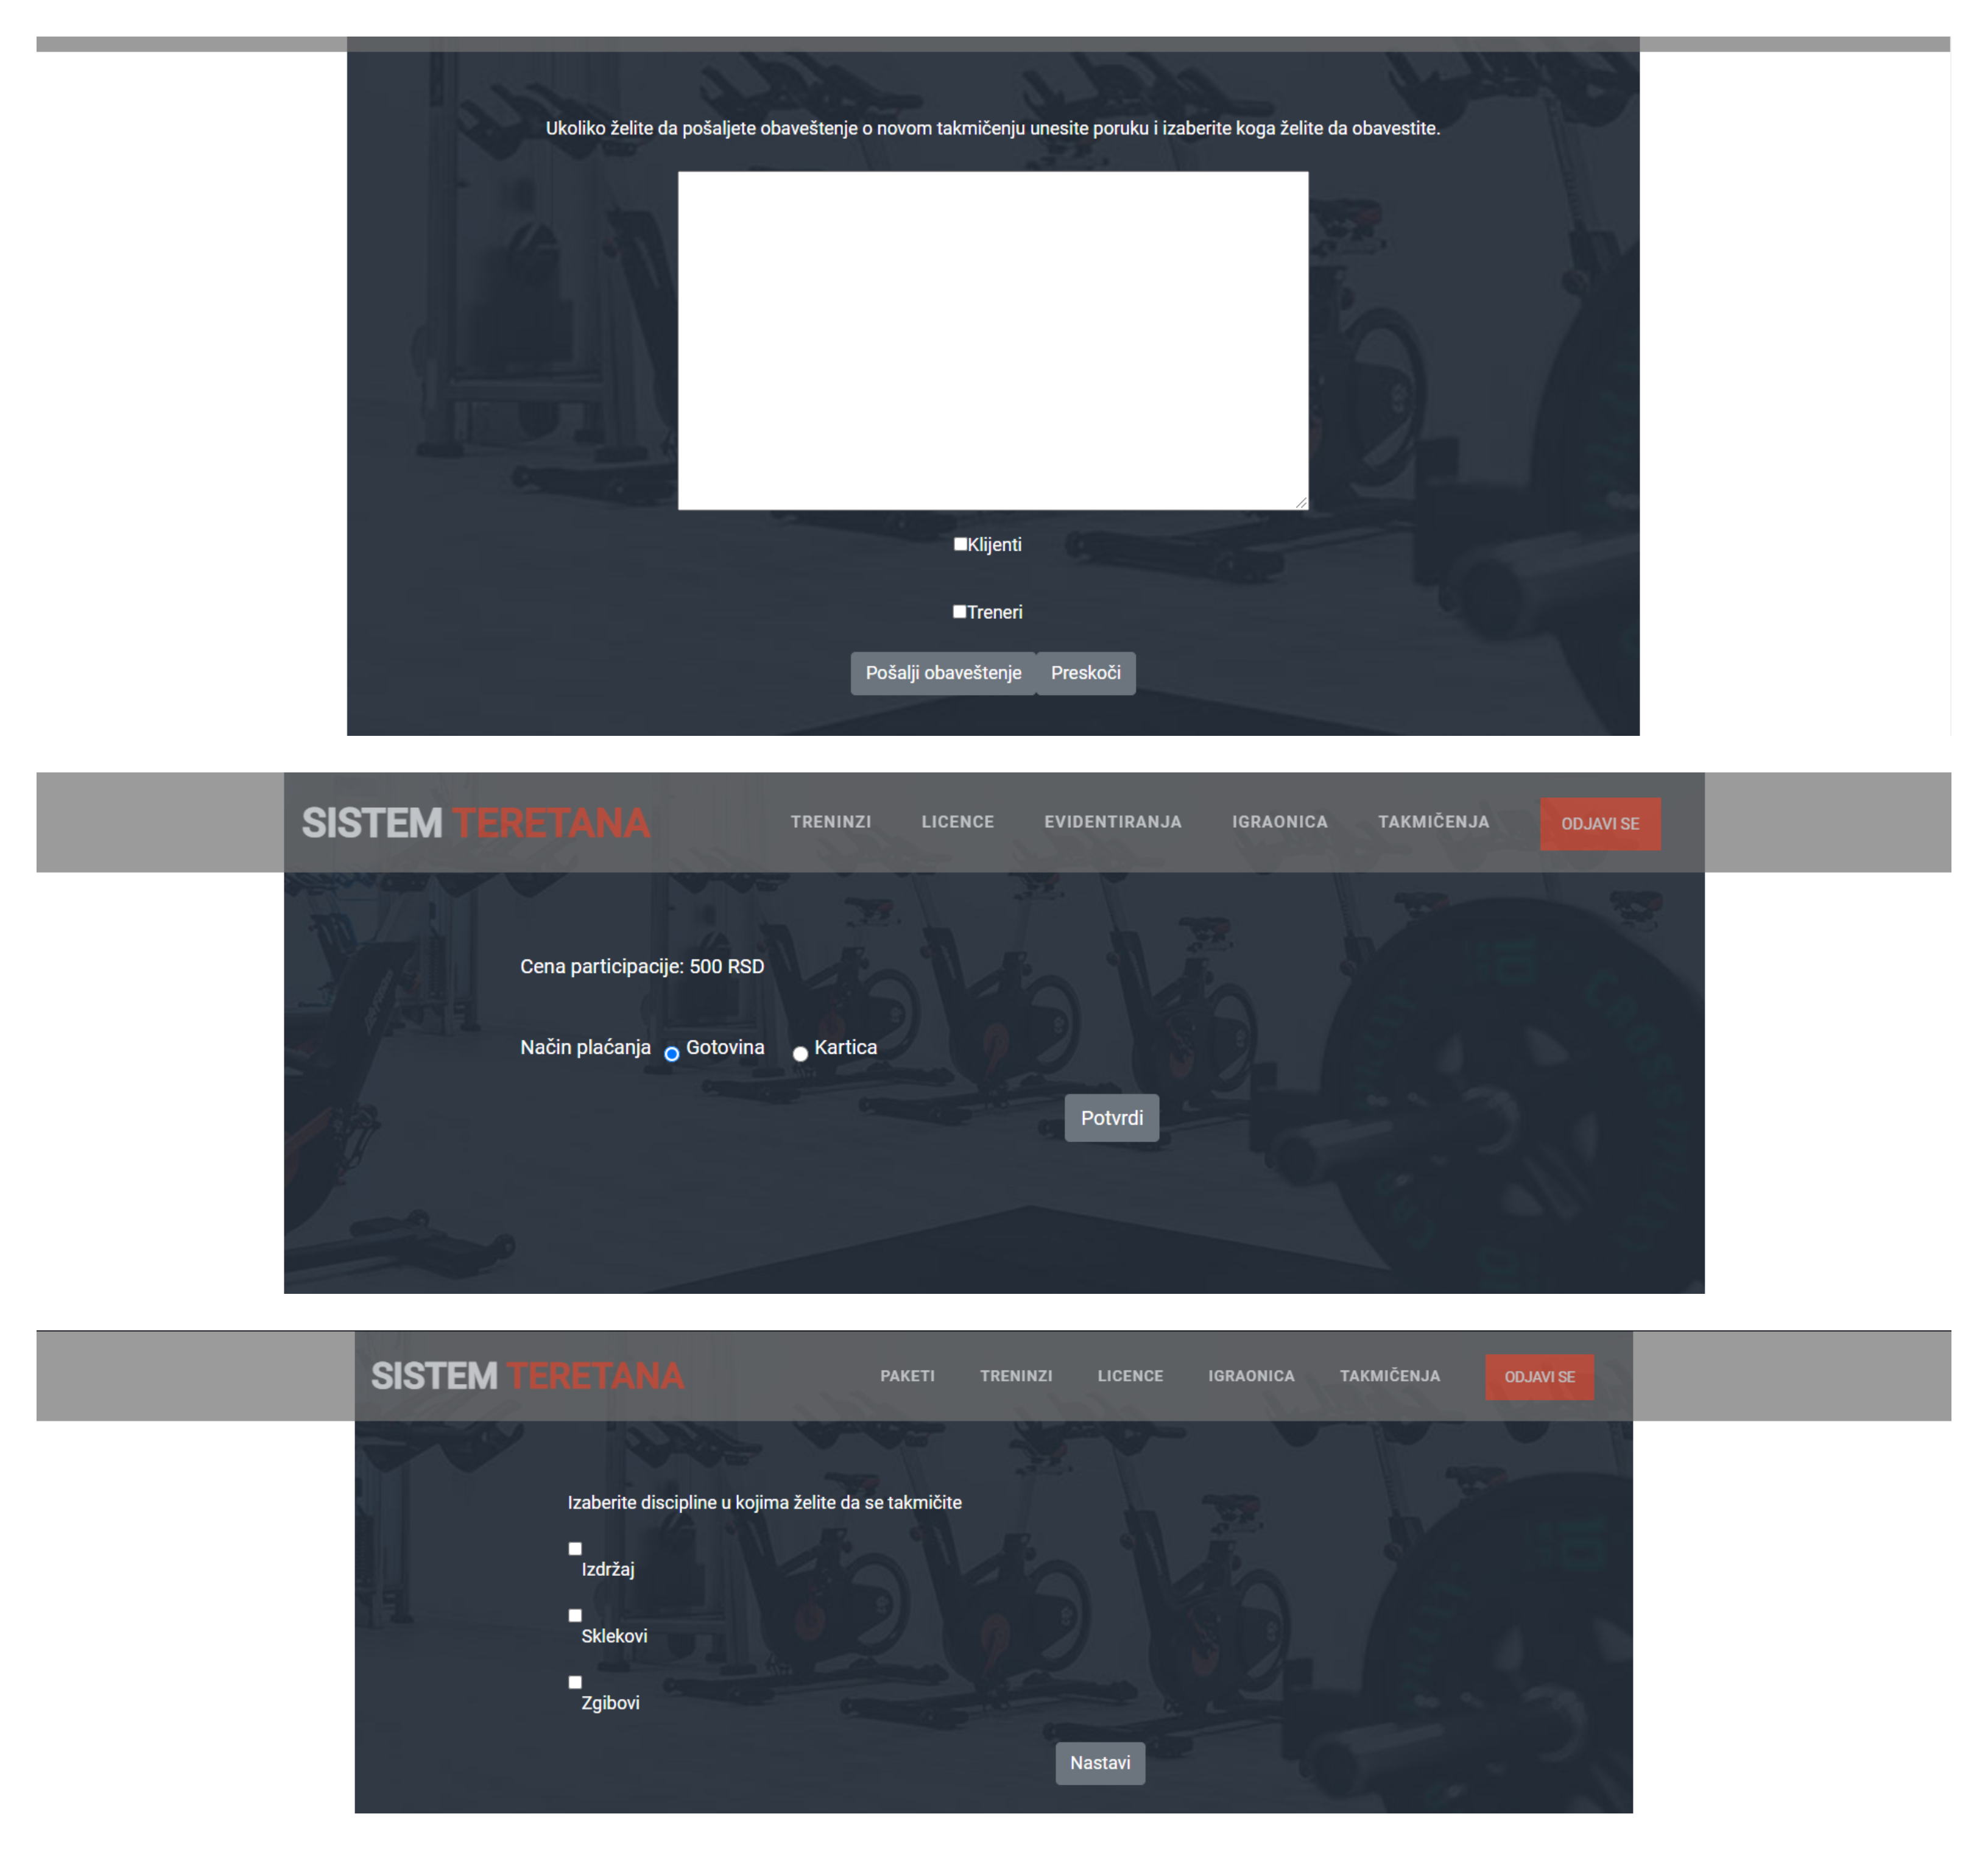
\includegraphics[scale=0.30]{sections/korisnicki_interfejs/screenshots/takmicenjaNovoIdisciplina.png}
\end{center}
\caption{Gore: Obaveštenje o novom takmičenju, Sredina: Izbor disciplina, Dole: Način plaćanja}
\label{fig:t_kreiranje_ob}
\end{figure}

Za otkazivanje takmičenja otvara se prozor za slanje propratnog obaveštenja sličan prethodno viđenom. On i formular za izmenu takmičenja mogu se videti na adresi navedenoj na kraju poglavlja.

Klijent vidi prikaz kao na slici (\ref{fig:takmicenja_uglovi} prva). Ukoliko želi da odustane od takmičenja dovoljno je da pritisne dugme, a klikom na Prijavi se otvara se formular (\ref{fig:t_kreiranje_ob} sredina) za izbor disciplina i pritiskom na Nastavi vodi se na deo za plaćanja. 

Recepcionar vidi (\ref{fig:takmicenja_uglovi} sredina) u polju za pretragu može da pronađe takmičara i odjavi ga sa takmičenja, a klikom na Prijavi novog takmičara otvara mu se formular \ref{fig:t_prijaviT}. Nakon prijave otvara mu se prozor za unos načina uplate.

\begin{figure}[!ht]
\begin{center}
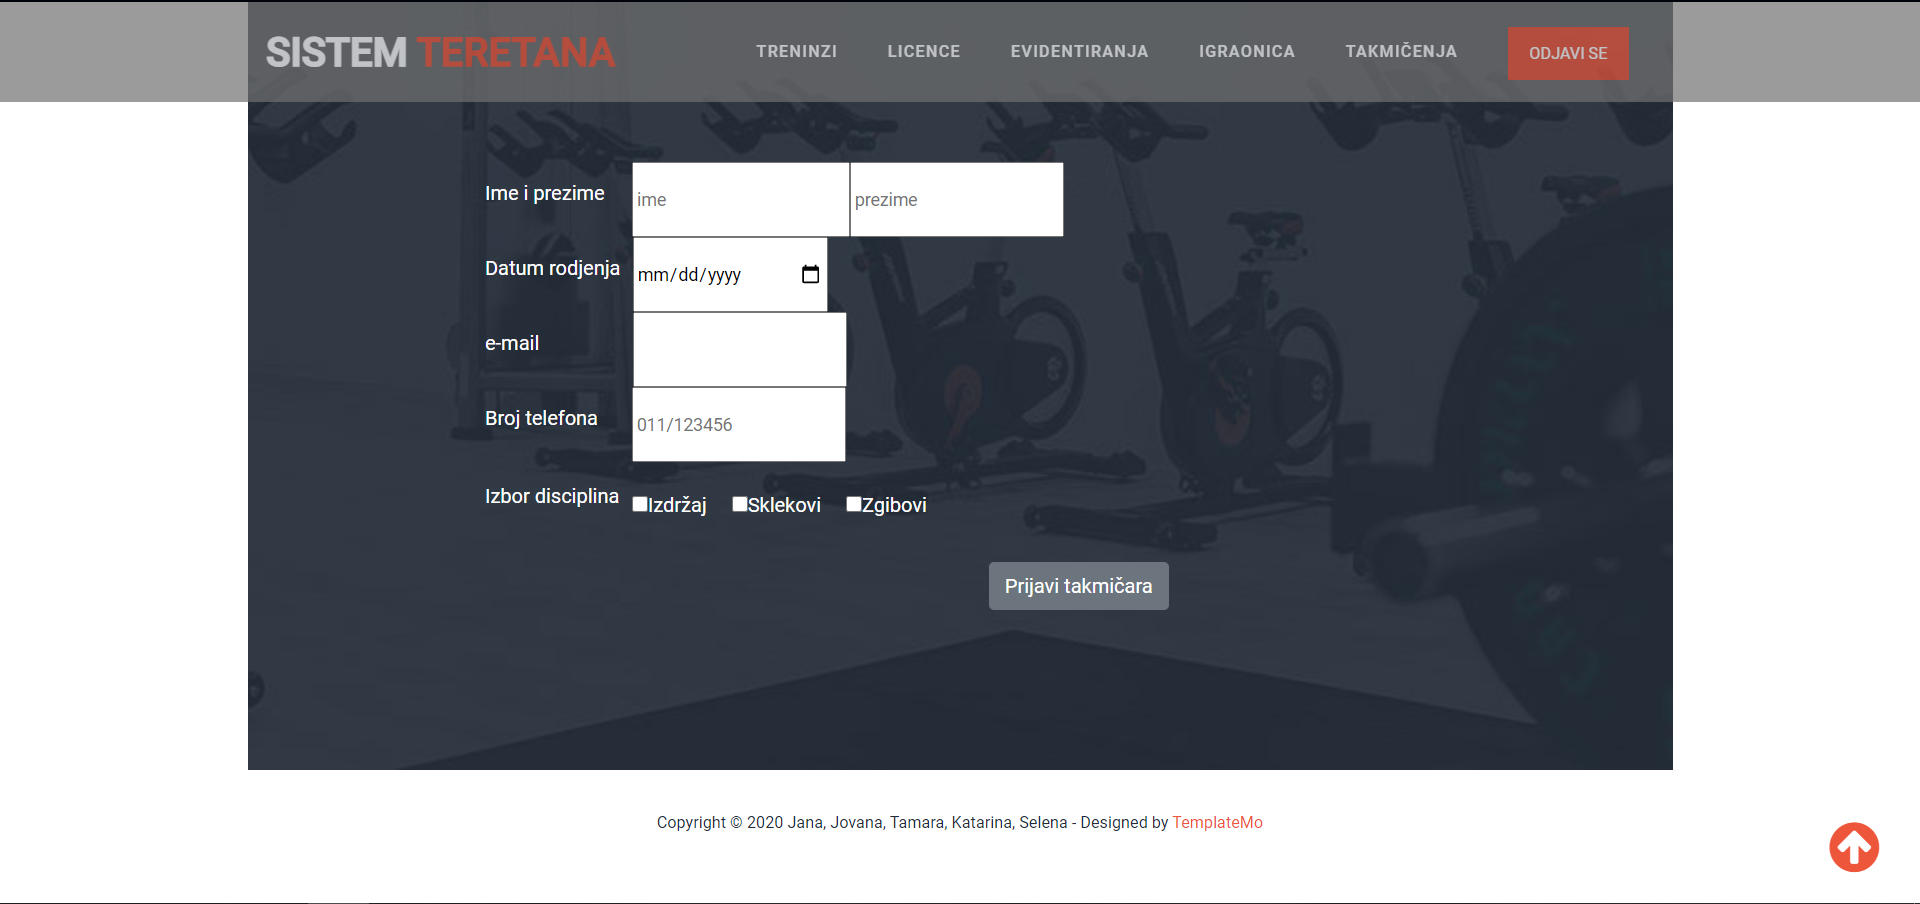
\includegraphics[scale=0.30]{sections/korisnicki_interfejs/screenshots/takmicenja_prijavi_takmicara.PNG}
\end{center}
\caption{Prijava takmičara}
\label{fig:t_prijaviT}
\end{figure}

\end{document}

